% !TeX program = xelatex
\documentclass[12pt,a4paper]{article}
\usepackage{fontspec}
\setmainfont{Times New Roman}[Path=C:/Windows/Fonts/,UprightFont=times.ttf,BoldFont=timesbd.ttf,ItalicFont=timesi.ttf,BoldItalicFont=timesbi.ttf]
\usepackage{amsmath,amssymb,amsfonts}
\usepackage[left=1.5cm,right=1.5cm,top=1.4cm,bottom=1.6cm,headheight=17pt]{geometry}
\usepackage{enumitem,array,graphicx,tikz,fancyhdr,needspace}
\usetikzlibrary{arrows.meta,calc,patterns}
% Sửa số đề và số trang đề thực tế sau khi biên dịch/tách PDF.
\newcommand{\soDe}{9}
\newcommand{\soTrangDe}{4}
\newcommand{\maDe}{\ifnum\soDe<1000 0\fi\ifnum\soDe<100 0\fi\ifnum\soDe<10 0\fi\soDe}
\pagestyle{fancy}
\fancyhf{}
\lhead{\small\textbf{ÔN TẬP GIỮA KÌ I}}
\rhead{\small\textit{Biên soạn: Dương Gia Bảo}}
\rfoot{\small Trang \thepage/\soTrangDe\ - Mã đề: \maDe}
\renewcommand{\headrulewidth}{0.4pt}
\fancypagestyle{answers}{\rfoot{\small Trang \thepage\ - Mã đề: \maDe}}
\fancypagestyle{firstpage}{\fancyhead{}\renewcommand{\headrulewidth}{0pt}}
\setlength{\parindent}{0pt}
\setlength{\parskip}{2.5pt}
\setlength{\emergencystretch}{1em}
\setlist[enumerate,1]{label=\textbf{Câu \arabic*:},leftmargin=*,itemsep=5pt,topsep=2pt}
\setlist[enumerate,2]{label=\alph*),leftmargin=*,itemsep=2pt,topsep=2pt}
\newcommand{\bonpa}[4]{\par\nobreak\smallskip\nobreak\noindent
\begin{tabular}{@{}p{0.47\linewidth}p{0.47\linewidth}@{}}
\textbf{A.} #1 & \textbf{B.} #2\\[8pt]
\textbf{C.} #3 & \textbf{D.} #4\end{tabular}}
\newcommand{\loigiai}[1]{\par\medskip\Needspace{4\baselineskip}\noindent\textbf{#1}\par\nobreak}
\newcommand{\otraloi}{\par\nobreak\smallskip\noindent\textit{Trả lời:}\quad\fbox{\rule{0pt}{11pt}\makebox[0.3cm]{}}\,\fbox{\rule{0pt}{11pt}\makebox[0.3cm]{}}\,\fbox{\rule{0pt}{11pt}\makebox[0.3cm]{}}\,\fbox{\rule{0pt}{11pt}\makebox[0.3cm]{}}}
\begin{document}
\thispagestyle{firstpage}
\noindent
\begin{minipage}[t]{0.35\textwidth}
    \centering
    {\fontsize{13}{15}\selectfont\textbf{ÔN TẬP GIỮA KÌ I}}\\[4pt]
    \textit{Biên soạn: Dương Gia Bảo}\\[5pt]
    \setlength{\fboxrule}{0.8pt}%
    \setlength{\fboxsep}{4pt}%
    \fbox{\begin{minipage}{0.83\linewidth}
        \centering
        {\fontsize{13}{15}\selectfont\textbf{ĐỀ ÔN TẬP}\\[2pt]\textbf{CHƯƠNG I VÀ II}}\\[4pt]
        \textit{(Đề thi gồm có \ifnum\soTrangDe<10 0\fi\soTrangDe\ trang)}
    \end{minipage}}
\end{minipage}\hfill
\begin{minipage}[t]{0.63\textwidth}
    \centering
    {\fontsize{13}{15}\selectfont\textbf{ÔN TẬP KIỂM TRA GIỮA KÌ I}\\[2pt]
    \textbf{NĂM HỌC 2026 - 2027}}\\[5pt]
    {\fontsize{14}{16}\selectfont\textbf{Môn: TOÁN - Lớp 12 (ĐỀ SỐ \soDe)}}\\[4pt]
    {\fontsize{11.5}{13}\selectfont\textit{Thời gian làm bài: 90 phút, không kể thời gian giao đề}}\\[5pt]
    \setlength{\fboxrule}{0.8pt}%
    \setlength{\fboxsep}{5pt}%
    \fbox{\makebox[3cm]{\fontsize{14}{16}\selectfont\textbf{Mã đề: \maDe}}}
\end{minipage}
\par\vspace{2pt}
\hrule height 0.6pt
\vspace{3pt}
\noindent\textit{Họ và tên học sinh:}\dotfill\hspace{1cm}\textit{Lớp:}\makebox[3.5cm]{\dotfill}
\par\vspace{2pt}
\hrule height 0.6pt
\vspace{3pt}

\section*{\large PHẦN I. Câu trắc nghiệm nhiều phương án lựa chọn}
\textit{Thí sinh trả lời từ câu 1 đến câu 12. Mỗi câu chỉ chọn một phương án.}
\begin{enumerate}
\item Cho hàm số $y=x^3-3x^2+2$. Hàm số đã cho nghịch biến trên khoảng nào dưới đây?
\bonpa{$(-\infty;0)$.}{$(0;2)$.}{$(2;+\infty)$.}{$(-2;2)$.}

\item Cho hàm số $y=-x^3+3x^2+9x-1$. Điểm cực đại của hàm số đã cho là
\bonpa{$x=-1$.}{$x=26$.}{$x=-6$.}{$x=3$.}

\item Giá trị lớn nhất của hàm số $f(x)=\dfrac{2x+1}{x-1}$ trên đoạn $[2;4]$ bằng
\bonpa{$5$.}{$3$.}{$\dfrac{5}{3}$.}{$7$.}

\item Đường tiệm cận đứng và đường tiệm cận ngang của đồ thị hàm số $y=\dfrac{3x-1}{x+2}$ lần lượt có phương trình là
\bonpa{$x=2$ và $y=3$.}{$x=-2$ và $y=-1$.}{$x=-2$ và $y=3$.}{$x=3$ và $y=-2$.}

\item Đường tiệm cận xiên của đồ thị hàm số $y=\dfrac{x^2-3x+4}{x-1}$ có phương trình là
\bonpa{$y=x-2$.}{$y=x-3$.}{$y=x+1$.}{$y=2x-1$.}

\item Đường cong trong hình vẽ bên là đồ thị của hàm số nào dưới đây?
\par\nobreak\smallskip
\begin{minipage}[c]{0.62\linewidth}
\bonpa{$y=\dfrac{x^2-x+1}{x-1}$.}{$y=\dfrac{x^2+2x-1}{x+1}$.}{$y=\dfrac{x^2+x-1}{x-1}$.}{$y=\dfrac{x^2-2x+2}{x-2}$.}
\end{minipage}\hfill
\begin{minipage}[c]{0.36\linewidth}\centering
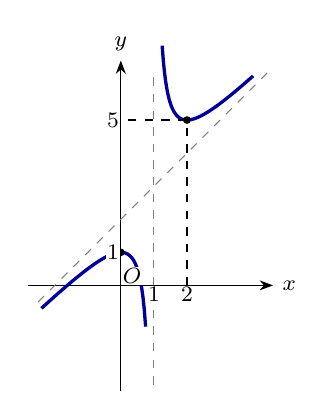
\begin{tikzpicture}[x=0.42cm,y=0.42cm,>=Stealth]
\draw[->] (-2.8,0)--(4.6,0) node[right] {\footnotesize $x$};
\draw[->] (0,-3.2)--(0,6.8) node[above] {\footnotesize $y$};
\draw[dashed,gray] (1,-3.0)--(1,6.5);
\draw[dashed,gray] (-2.5,-0.5)--(4.5,6.5);
\draw[very thick,blue!60!black,domain=-2.4:0.75,samples=80] plot (\x,{(\x*\x+\x-1)/(\x-1)});
\draw[very thick,blue!60!black,domain=1.25:4.0,samples=80] plot (\x,{(\x*\x+\x-1)/(\x-1)});
\draw[dashed] (2,0)--(2,5)--(0,5);
\fill (0,1) circle (1.4pt);
\fill (2,5) circle (1.4pt);
\node[above right,fill=white,inner sep=0.5pt] at (0,0) {\footnotesize $O$};
\node[below,fill=white,inner sep=0.5pt] at (1,0) {\footnotesize $1$};
\node[below,fill=white,inner sep=0.5pt] at (2,0) {\footnotesize $2$};
\node[left,fill=white,inner sep=0.5pt] at (0,1) {\footnotesize $1$};
\node[left,fill=white,inner sep=0.5pt] at (0,5) {\footnotesize $5$};
\end{tikzpicture}
\end{minipage}
\end{enumerate}

\newpage
\begin{enumerate}[start=7]
\item Một công ty sản xuất bóng đèn LED ước tính chi phí sản xuất $x$ nghìn bóng đèn ($1\le x\le 20$) là $C(x)=x^2-10x+100$ (triệu đồng). Chi phí sản xuất trung bình cho mỗi nghìn chiếc bóng đèn là $\bar{C}(x)=\dfrac{C(x)}{x}=x-10+\dfrac{100}{x}$. Để chi phí sản xuất trung bình trên mỗi nghìn chiếc bóng đèn là thấp nhất thì công ty nên sản xuất bao nhiêu nghìn chiếc bóng đèn?
\bonpa{$5$.}{$8$.}{$12$.}{$10$.}

\item Cho tứ diện $ABCD$. Gọi $M$ và $N$ lần lượt là trung điểm của các cạnh $AB$ và $CD$. Khẳng định nào sau đây đúng?
\bonpa{$\vec{AC}+\vec{BD}=\vec{MN}$.}{$\vec{AC}+\vec{BD}=2\vec{MN}$.}{$\vec{AB}+\vec{CD}=2\vec{MN}$.}{$\vec{AD}+\vec{BC}=\vec{MN}$.}

\item Trong không gian $Oxyz$, cho điểm $M(2;-3;5)$. Hình chiếu vuông góc của điểm $M$ lên trục $Oz$ là điểm
\bonpa{$M_1(2;-3;0)$.}{$M_2(0;-3;5)$.}{$M_3(2;0;0)$.}{$M_4(0;0;5)$.}

\item Trong không gian $Oxyz$, cho hai vectơ $\vec{a}=(1;2;-1)$ và $\vec{b}=(-2;1;3)$. Tọa độ của vectơ $\vec{u}=2\vec{a}+\vec{b}$ là
\bonpa{$(0;5;1)$.}{$(-1;3;2)$.}{$(4;3;-5)$.}{$(0;5;-1)$.}

\item Trong không gian $Oxyz$, cho hai vectơ $\vec{u}=(2;-1;1)$ và $\vec{v}=(1;3;k)$. Giá trị của tham số $k$ để hai vectơ $\vec{u}$ và $\vec{v}$ vuông góc với nhau là
\bonpa{$k=-1$.}{$k=1$.}{$k=5$.}{$k=-5$.}

\item Trong không gian $Oxyz$, cho hai điểm $A(1;3;-2)$ và $B(3;5;-1)$. Độ dài đoạn thẳng $AB$ bằng
\bonpa{$\sqrt{5}$.}{$9$.}{$3$.}{$\sqrt{17}$.}
\end{enumerate}

\vspace{3pt}
\section*{\large PHẦN II. Câu trắc nghiệm đúng hoặc sai}
\textit{Thí sinh trả lời từ câu 1 đến câu 4. Trong mỗi ý a), b), c), d) ở mỗi câu, thí sinh chọn đúng hoặc sai.}
\begin{enumerate}
\item Cho hàm số $y=f(x)=\dfrac{x^2-x+2}{x+1}$.
\begin{enumerate}
\item Tập xác định của hàm số là $D=\mathbb{R}\setminus\{-1\}$.
\item Đạo hàm của hàm số là $f'(x)=\dfrac{x^2+2x-3}{(x+1)^2}$.
\item Đồ thị hàm số có đường tiệm cận xiên là đường thẳng $y=x+2$.
\item Đồ thị hàm số có hai điểm cực trị $A$ và $B$. Khoảng cách giữa hai điểm cực trị là $AB=4\sqrt{5}$.
\end{enumerate}
\end{enumerate}

\newpage
\begin{enumerate}[start=2]
\item Một xưởng sản xuất gốm sứ thủ công mỹ nghệ sản xuất $x$ trăm sản phẩm trong một tháng ($0 < x \le 40$). Tổng chi phí sản xuất (tính bằng triệu đồng) được cho bởi hàm số $C(x)=x^3-20x^2+500x+600$. Doanh thu từ việc bán sản phẩm (tính bằng triệu đồng) được cho bởi hàm số $R(x)=1400x-5x^2$. Lợi nhuận của xưởng sản xuất là $P(x)=R(x)-C(x)$.
\begin{enumerate}
\item Chi phí cố định ban đầu của xưởng (khi chưa sản xuất sản phẩm nào) là $600$ triệu đồng.
\item Doanh thu của xưởng khi bán được $10$ trăm sản phẩm là $13500$ triệu đồng.
\item Hàm lợi nhuận của xưởng theo số lượng $x$ là $P(x)=-x^3+15x^2+900x-600$.
\item Xưởng đạt lợi nhuận lớn nhất trong tháng khi sản xuất $25$ trăm sản phẩm.
\end{enumerate}

\item Trong không gian $Oxyz$, cho ba điểm $A(1;0;2)$, $B(3;1;0)$ và $C(2;2;4)$.
\begin{enumerate}
\item Tọa độ của vectơ $\vec{AB}$ là $\vec{AB}=(2;1;-2)$.
\item Trọng tâm $G$ của tam giác $ABC$ có tọa độ là $G(2;1;2)$.
\item Tích vô hướng $\vec{AB}\cdot\vec{AC}=0$, suy ra tam giác $ABC$ vuông tại $A$.
\item Tọa độ điểm $D$ để tứ giác $ABCD$ là hình bình hành là $D(4;3;2)$.
\end{enumerate}

\item Một chùm đèn nghệ thuật hình chóp được treo ở sảnh triển lãm gồm một móc treo chính $S$ gắn cố định trên trần nhà. Từ móc $S$, có ba sợi cáp chịu lực có độ dài bằng nhau $SA=SB=SC=2\sqrt{3}\text{ m}$ treo ba bóng đèn nghệ thuật tại ba vị trí $A, B, C$. Góc tạo bởi các sợi cáp tại đỉnh $S$ lần lượt là $\widehat{ASB}=60^\circ$, $\widehat{BSC}=90^\circ$ và $\widehat{CSA}=120^\circ$. Gọi $G$ là trọng tâm của tam giác $ABC$. Người ta lắp thêm một thanh kim loại nối từ đỉnh $S$ đến trọng tâm $G$ để dẫn dây điện và ổn định kết cấu.
\begin{enumerate}
\item Tích vô hướng $\vec{SA}\cdot\vec{SB}=6$.
\item Vì $G$ là trọng tâm tam giác $ABC$ nên $\vec{SG}=\dfrac{1}{3}(\vec{SA}+\vec{SB}+\vec{SC})$.
\item Tích vô hướng $\vec{SA}\cdot\vec{SC}=6$.
\item Chiều dài của thanh kim loại $SG$ bằng $2\text{ m}$.
\end{enumerate}
\end{enumerate}

\vspace{3pt}
\section*{\large PHẦN III. Câu trắc nghiệm trả lời ngắn}
\textit{Thí sinh trả lời từ câu 1 đến câu 6. Mỗi câu trả lời đúng thí sinh được 0,5 điểm.}
\begin{enumerate}
\item Tìm số giá trị nguyên của tham số $m\in[-10;10]$ để hàm số $y=\dfrac{1}{3}x^3-mx^2+(2m+3)x+1$ đồng biến trên khoảng $(-\infty;+\infty)$.
\otraloi

\item Trong không gian $Oxyz$, cho hình hộp $ABCD.A'B'C'D'$ có tọa độ các đỉnh $A(1;1;0)$, $B(2;3;1)$, $D(-1;2;2)$ và $A'(3;1;2)$. Tìm tọa độ đỉnh $C'(x;y;z)$, sau đó tính giá trị biểu thức $T=x+y+z$.
\otraloi
\end{enumerate}

\newpage
\begin{enumerate}[start=3]
\item Cho hàm số $y=\dfrac{x^2-5x+7}{x-1}$ có đồ thị $(C)$. Đường tiệm cận xiên của $(C)$ cắt hai trục tọa độ $Ox, Oy$ lần lượt tại hai điểm $P$ và $Q$. Tính diện tích tam giác $OPQ$ (với $O$ là gốc tọa độ).
\otraloi

\item Trong không gian $Oxyz$ (với đơn vị đo trên các trục là mét), có hai thiết bị bay không người lái (drone) đang bay thử nghiệm. Tại thời điểm $t$ giây ($t\ge 0$), vị trí của drone thứ nhất là $A(t;2;10)$ và vị trí của drone thứ hai là $B(2t+5;2t+3;2t+2)$. Khoảng cách ngắn nhất giữa hai drone trong quá trình bay bằng bao nhiêu mét?
\otraloi

\item Người ta muốn cắt một tấm tôn hình chữ nhật có kích thước $50\text{ cm}\times 80\text{ cm}$ để gập thành một chiếc hộp chứa đồ không nắp dạng hình hộp chữ nhật. Người ta cắt bỏ ở bốn góc bốn hình vuông bằng nhau có cạnh bằng $x\text{ cm}$ rồi gập bốn mép xung quanh lên (hình vẽ minh họa). Tìm giá trị của $x$ (theo xentimét) để thể tích của chiếc hộp nhận được là lớn nhất.
\begin{center}
\begin{tikzpicture}[x=0.72cm,y=0.72cm,>=Stealth]
\draw[thick] (0,0) rectangle (6,3.75);
% Cắt 4 góc
\fill[gray!25] (0,0) rectangle (0.8,0.8);
\fill[gray!25] (5.2,0) rectangle (6,0.8);
\fill[gray!25] (0,2.95) rectangle (0.8,3.75);
\fill[gray!25] (5.2,2.95) rectangle (6,3.75);

\draw[thick] (0.8,0)--(0.8,0.8)--(0,0.8);
\draw[thick] (5.2,0)--(5.2,0.8)--(6,0.8);
\draw[thick] (0,2.95)--(0.8,2.95)--(0.8,3.75);
\draw[thick] (5.2,3.75)--(5.2,2.95)--(6,2.95);

% Nếp gấp nét đứt
\draw[dashed,thick,blue!70!black] (0.8,0.8)--(5.2,0.8);
\draw[dashed,thick,blue!70!black] (0.8,2.95)--(5.2,2.95);
\draw[dashed,thick,blue!70!black] (0.8,0.8)--(0.8,2.95);
\draw[dashed,thick,blue!70!black] (5.2,0.8)--(5.2,2.95);

% Kích thước
\draw[<->] (0,-0.35)--(6,-0.35) node[midway,below] {\footnotesize $80\text{ cm}$};
\draw[<->] (-0.35,0)--(-0.35,3.75) node[midway,left] {\footnotesize $50\text{ cm}$};
\draw[<->] (0.8,0.4)--(0,0.4) node[midway,above] {\footnotesize $x$};
\draw[<->] (0.4,0.8)--(0.4,0) node[midway,right] {\footnotesize $x$};

\node at (3,1.87) {\footnotesize\textit{Đáy hộp}};
\end{tikzpicture}
\par\smallskip{\footnotesize\textit{Hình minh họa tấm tôn và các góc vuông bị cắt bỏ.}}
\end{center}
\otraloi

\item Một giàn khoan dầu khí $A$ nằm trên biển cách đường bờ biển thẳng một khoảng $AH=6\text{ km}$ ($H$ là hình chiếu vuông góc của $A$ lên bờ biển). Nhà máy lọc dầu $B$ nằm trên bờ biển và cách điểm $H$ một khoảng $HB=13\text{ km}$. Người ta dự định xây dựng một hệ thống đường ống dẫn dầu nối từ giàn khoan $A$ đến nhà máy $B$ gồm hai đoạn: đoạn ống ngầm dưới biển nối từ $A$ đến trạm tiếp nhận $C$ trên bờ biển ($C$ nằm giữa $H$ và $B$), và đoạn đường ống chạy dọc theo bờ biển nối từ $C$ đến $B$ (hình vẽ minh họa). Biết chi phí lắp đặt mỗi kilômét ống ngầm dưới biển là $5$ tỷ đồng, chi phí lắp đặt mỗi kilômét đường ống trên bờ là $4$ tỷ đồng. Tổng chi phí nhỏ nhất để lắp đặt toàn bộ hệ thống đường ống dẫn dầu này bằng bao nhiêu tỷ đồng?
\begin{center}
\begin{tikzpicture}[x=0.68cm,y=0.68cm,>=Stealth]
\draw[thick,blue!50!gray] (-0.5,0)--(11.5,0) node[above,black] {\footnotesize Đường bờ biển};
\fill[cyan!10] (-0.5,-2.7) rectangle (11.5,0);
\node at (4.5,-1.9) {\textit{\footnotesize Biển}};
\node at (4.5,0.7) {\textit{\footnotesize Đất liền}};

\coordinate (A) at (1.5,-2.3);
\coordinate (H) at (1.5,0);
\coordinate (C) at (7.0,0);
\coordinate (B) at (10.5,0);

\fill (A) circle (2pt) node[below] {$A$ (Giàn khoan)};
\fill (H) circle (2pt) node[above] {$H$};
\fill (C) circle (2pt) node[above] {$C$};
\fill (B) circle (2pt) node[above] {$B$ (Nhà máy)};

\draw[dashed] (A)--(H);
\draw (1.5,-0.3)--(1.8,-0.3)--(1.8,0);
\draw[line width=1.4pt,red!80!black] (A)--(C) node[midway,below right] {\footnotesize Ống ngầm};
\draw[line width=1.5pt,orange!80!black] (C)--(B) node[midway,above] {\footnotesize Ống trên bờ};

\draw[<->] (1.5,0.4)--(10.5,0.4) node[midway,above] {\footnotesize $13\text{ km}$};
\draw[<->] (1.0,0)--(1.0,-2.3) node[midway,left] {\footnotesize $6\text{ km}$};
\draw[<->] (1.5,-0.3)--(7.0,-0.3) node[midway,below] {\footnotesize $x$};
\end{tikzpicture}
\par\smallskip{\footnotesize\textit{Sơ đồ phương án đặt đường ống dẫn dầu.}}
\end{center}
\otraloi
\end{enumerate}
\begin{center}\textbf{---------------- HẾT ----------------}\end{center}

\newpage\pagestyle{answers}
\begin{center}\Large\textbf{BẢNG ĐÁP ÁN TỔNG HỢP}\end{center}
\textbf{Phần I. Trắc nghiệm nhiều phương án lựa chọn}
\begin{center}
\renewcommand{\arraystretch}{1.5}
\begin{tabular}{|c|*{12}{c|}}\hline
Câu & 1&2&3&4&5&6&7&8&9&10&11&12\\\hline
Đáp án & B & D & A & C & A & C & D & B & D & A & B & C \\\hline
\end{tabular}
\end{center}

\textbf{Phần II. Đúng hoặc sai}
\begin{center}
\renewcommand{\arraystretch}{1.4}
\begin{tabular}{|c|c|c|c|c|}\hline
Câu & a) & b) & c) & d)\\\hline
1 & Đ & Đ & S & Đ\\\hline
2 & Đ & Đ & Đ & S\\\hline
3 & Đ & Đ & Đ & S\\\hline
4 & Đ & Đ & S & Đ\\\hline
\end{tabular}
\end{center}

\textbf{Phần III. Trả lời ngắn}
\begin{center}
\renewcommand{\arraystretch}{1.5}
\begin{tabular}{|c|c|c|c|c|c|c|}\hline
Câu & 1 & 2 & 3 & 4 & 5 & 6\\\hline
Đáp án & 5 & 11 & 8 & 9 & 10 & 70 \\\hline
\end{tabular}
\end{center}

\vspace{0.5cm}
\begin{center}
\large\textbf{HƯỚNG DẪN GIẢI CHI TIẾT}
\end{center}

\section*{PHẦN I}

\loigiai{Câu 1. Chọn B.}
Hàm số đã cho là $y=x^3-3x^2+2$.
Tập xác định: $D=\mathbb{R}$.
Đạo hàm: $y'=3x^2-6x=3x(x-2)$.
Ta có $y'<0 \iff 3x(x-2)<0 \iff 0<x<2$.
Do đó, hàm số nghịch biến trên khoảng $(0;2)$.

\loigiai{Câu 2. Chọn D.}
Hàm số đã cho là $y=-x^3+3x^2+9x-1$.
Tập xác định: $D=\mathbb{R}$.
Đạo hàm: $y'=-3x^2+6x+9=-3(x^2-2x-3)=-3(x-3)(x+1)$.
$y'=0 \iff x=-1$ hoặc $x=3$.
Đạo hàm cấp hai: $y''=-6x+6$.
Tại $x=3$: $y''(3)=-6(3)+6=-12<0 \implies x=3$ là điểm cực đại của hàm số.

\loigiai{Câu 3. Chọn A.}
Hàm số $f(x)=\dfrac{2x+1}{x-1}$ liên tục trên đoạn $[2;4]$.
Đạo hàm: $f'(x)=\dfrac{2(x-1)-(2x+1)(1)}{(x-1)^2}=\dfrac{-3}{(x-1)^2}<0,\;\forall x\in[2;4]$.
Do hàm số nghịch biến trên $[2;4]$ nên giá trị lớn nhất của hàm số đạt tại đầu mút bên trái:
$\max_{[2;4]} f(x)=f(2)=\dfrac{2(2)+1}{2-1}=5$.

\loigiai{Câu 4. Chọn C.}
Hàm số $y=\dfrac{3x-1}{x+2}$.
Tập xác định: $D=\mathbb{R}\setminus\{-2\}$.
Vì $\lim_{x\to (-2)^+} \dfrac{3x-1}{x+2}=-\infty$ nên đường thẳng $x=-2$ là tiệm cận đứng của đồ thị hàm số.
Vì $\lim_{x\to +\infty} \dfrac{3x-1}{x+2}=3$ nên đường thẳng $y=3$ là tiệm cận ngang của đồ thị hàm số.

\loigiai{Câu 5. Chọn A.}
Hàm số $y=\dfrac{x^2-3x+4}{x-1}$.
Biến đổi tử thức: $x^2-3x+4 = x(x-1) - 2(x-1) + 2 = (x-2)(x-1)+2$.
Do đó: $y=x-2+\dfrac{2}{x-1}$.
Ta có $\lim_{x\to\pm\infty}[y-(x-2)]=\lim_{x\to\pm\infty}\dfrac{2}{x-1}=0$.
Vậy đường tiệm cận xiên của đồ thị hàm số có phương trình là $y=x-2$.

\loigiai{Câu 6. Chọn C.}
Quan sát đồ thị hàm số ta thấy:
- Đồ thị có tiệm cận đứng là đường thẳng $x=1$, tiệm cận xiên là đường thẳng $y=x+2$.
- Đồ thị cắt trục tung tại điểm $(0;1)$ và có điểm cực tiểu tại $(2;5)$.
Xét các hàm số đã cho:
Chỉ có hàm số $y=\dfrac{x^2+x-1}{x-1}=x+2+\dfrac{1}{x-1}$ thỏa mãn:
+ Mẫu số triệt tiêu tại $x=1 \implies x=1$ là tiệm cận đứng.
+ $y-(x+2)=\dfrac{1}{x-1}\to 0$ khi $x\to\pm\infty \implies y=x+2$ là tiệm cận xiên.
+ Tại $x=0$, $y=1$.
+ Tại $x=2$, $y=\dfrac{4+2-1}{1}=5$.
Vậy đường cong là đồ thị của hàm số $y=\dfrac{x^2+x-1}{x-1}$.

\loigiai{Câu 7. Chọn D.}
Hàm chi phí sản xuất trung bình là $\bar{C}(x)=x-10+\dfrac{100}{x}$ với $x\in[1;20]$.
Đạo hàm: $\bar{C}'(x)=1-\dfrac{100}{x^2}=\dfrac{x^2-100}{x^2}$.
Cho $\bar{C}'(x)=0 \iff x^2=100 \iff x=10$ (do $x\in[1;20]$).
Bảng biến thiên cho thấy $\bar{C}(x)$ nghịch biến trên $(0;10)$ và đồng biến trên $(10;20)$.
Do đó, $\bar{C}(x)$ đạt giá trị nhỏ nhất tại $x=10$.
Vậy công ty nên sản xuất $10$ nghìn chiếc bóng đèn.

\loigiai{Câu 8. Chọn B.}
Gọi $M, N$ lần lượt là trung điểm của $AB$ và $CD$.
Theo quy tắc xen điểm, ta có:
$\vec{AC}=\vec{AM}+\vec{MN}+\vec{NC}$,
$\vec{BD}=\vec{BM}+\vec{MN}+\vec{ND}$.
Cộng vế với vế hai đẳng thức trên:
$\vec{AC}+\vec{BD}=2\vec{MN}+(\vec{AM}+\vec{BM})+(\vec{NC}+\vec{ND})$.
Vì $M$ là trung điểm $AB$ và $N$ là trung điểm $CD$ nên $\vec{AM}+\vec{BM}=\vec{0}$ và $\vec{NC}+\vec{ND}=\vec{0}$.
Do đó, $\vec{AC}+\vec{BD}=2\vec{MN}$.

\loigiai{Câu 9. Chọn D.}
Trong không gian $Oxyz$, hình chiếu vuông góc của điểm $M(x_0;y_0;z_0)$ lên trục $Oz$ có tọa độ là $(0;0;z_0)$.
Với $M(2;-3;5)$, hình chiếu vuông góc của $M$ lên trục $Oz$ là điểm $M_4(0;0;5)$.

\loigiai{Câu 10. Chọn A.}
Ta có: $2\vec{a}=2(1;2;-1)=(2;4;-2)$.
Do đó: $\vec{u}=2\vec{a}+\vec{b}=(2+(-2);\; 4+1;\; -2+3)=(0;5;1)$.

\loigiai{Câu 11. Chọn B.}
Hai vectơ $\vec{u}=(2;-1;1)$ và $\vec{v}=(1;3;k)$ vuông góc với nhau khi và chỉ khi:
$\vec{u}\cdot\vec{v}=0 \iff 2\cdot 1 + (-1)\cdot 3 + 1\cdot k = 0 \iff 2-3+k=0 \iff k=1$.

\loigiai{Câu 12. Chọn C.}
Độ dài đoạn thẳng $AB$ là:
$AB=\sqrt{(3-1)^2+(5-3)^2+(-1-(-2))^2}=\sqrt{4+4+1}=3$.

\section*{PHẦN II}

\loigiai{Câu 1.}
Cho hàm số $y=f(x)=\dfrac{x^2-x+2}{x+1}$.
a) Hàm số xác định khi và chỉ khi $x+1\ne 0 \iff x\ne -1$. Do đó tập xác định là $D=\mathbb{R}\setminus\{-1\}$. Ý a) \textbf{ĐÚNG}.\\
b) Ta có $f'(x)=\dfrac{(2x-1)(x+1)-(x^2-x+2)(1)}{(x+1)^2}=\dfrac{(2x^2+x-1)-(x^2-x+2)}{(x+1)^2}=\dfrac{x^2+2x-3}{(x+1)^2}$. Ý b) \textbf{ĐÚNG}.\\
c) Ta có $f(x)=\dfrac{(x-2)(x+1)+4}{x+1}=x-2+\dfrac{4}{x+1}$.
Vì $\lim_{x\to\pm\infty}[f(x)-(x-2)]=0$ nên đường tiệm cận xiên của đồ thị hàm số là đường thẳng $y=x-2$, không phải $y=x+2$. Ý c) \textbf{SAI}.\\
d) $f'(x)=0 \iff x^2+2x-3=0 \iff x=1$ hoặc $x=-3$.
Với $x=1 \implies y=1$, ta có điểm cực trị thứ nhất $A(1;1)$.
Với $x=-3 \implies y=-7$, ta có điểm cực trị thứ hai $B(-3;-7)$.
Khoảng cách giữa hai điểm cực trị là:
$AB=\sqrt{(-3-1)^2+(-7-1)^2}=\sqrt{(-4)^2+(-8)^2}=\sqrt{16+64}=\sqrt{80}=4\sqrt{5}$. Ý d) \textbf{ĐÚNG}.

\loigiai{Câu 2.}
a) Chi phí cố định ban đầu của xưởng là chi phí khi chưa sản xuất sản phẩm nào ($x=0$):
$C(0)=0^3-20(0)^2+500(0)+600=600$ triệu đồng. Ý a) \textbf{ĐÚNG}.\\
b) Khi bán được $10$ trăm sản phẩm ($x=10$):
$R(10)=1400(10)-5(10)^2=14000-500=13500$ triệu đồng. Ý b) \textbf{ĐÚNG}.\\
c) Hàm lợi nhuận của xưởng là:
$P(x)=R(x)-C(x)=(1400x-5x^2)-(x^3-20x^2+500x+600)=-x^3+15x^2+900x-600$. Ý c) \textbf{ĐÚNG}.\\
d) Xét hàm số $P(x)$ trên khoảng $(0;40]$:
Đạo hàm: $P'(x)=-3x^2+30x+900=-3(x^2-10x-300)=-3(x-20)(x+15)$.
Cho $P'(x)=0$ trên $(0;40] \iff x=20$.
Vì $P''(x)=-6x+30$ nên $P''(20)=-120+30=-90<0$, suy ra $P(x)$ đạt cực đại và cũng là giá trị lớn nhất tại $x=20$ trăm sản phẩm (tương ứng với $2000$ sản phẩm).
Khẳng định lợi nhuận lớn nhất khi sản xuất $25$ trăm sản phẩm là sai. Ý d) \textbf{SAI}.

\loigiai{Câu 3.}
Trong không gian $Oxyz$, cho $A(1;0;2)$, $B(3;1;0)$ và $C(2;2;4)$.\\
a) Tọa độ của vectơ $\vec{AB}$ là:
$\vec{AB}=(3-1;\; 1-0;\; 0-2)=(2;1;-2)$. Ý a) \textbf{ĐÚNG}.\\
b) Trọng tâm $G$ của tam giác $ABC$ có tọa độ:
$x_G=\dfrac{1+3+2}{3}=2$, $y_G=\dfrac{0+1+2}{3}=1$, $z_G=\dfrac{2+0+4}{3}=2$.
Vậy $G(2;1;2)$. Ý b) \textbf{ĐÚNG}.\\
c) Ta có $\vec{AC}=(2-1;\; 2-0;\; 4-2)=(1;2;2)$.
Tích vô hướng: $\vec{AB}\cdot\vec{AC}=2\cdot 1 + 1\cdot 2 + (-2)\cdot 2 = 2+2-4=0$.
Suy ra $\vec{AB}\perp\vec{AC}$, hay tam giác $ABC$ vuông tại $A$. Ý c) \textbf{ĐÚNG}.\\
d) Tứ giác $ABCD$ là hình bình hành khi và chỉ khi $\vec{AB}=\vec{DC} \iff C-D=\vec{AB} \iff D=C-\vec{AB}$.
Tọa độ điểm $D$: $x_D=2-2=0$, $y_D=2-1=1$, $z_D=4-(-2)=6 \implies D(0;1;6)$.
Điểm $(4;3;2)$ tương ứng với đỉnh thứ tư của hình bình hành $ABDC$ (khi $\vec{AD}=\vec{AB}+\vec{AC}$). Ý d) \textbf{SAI}.

\loigiai{Câu 4.}
Móc treo $S$ có ba sợi cáp $SA=SB=SC=2\sqrt{3}\text{ m}$.\\
a) Ta có $\vec{SA}\cdot\vec{SB}=|\vec{SA}|\cdot|\vec{SB}|\cos\widehat{ASB}=(2\sqrt{3})(2\sqrt{3})\cos 60^\circ=12\cdot\dfrac{1}{2}=6$. Ý a) \textbf{ĐÚNG}.\\
b) Do $G$ là trọng tâm của tam giác $ABC$, theo hệ thức vectơ trọng tâm cơ bản với điểm $S$ bất kì, ta luôn có:
$\vec{SG}=\dfrac{1}{3}(\vec{SA}+\vec{SB}+\vec{SC})$. Ý b) \textbf{ĐÚNG}.\\
c) Ta có $\vec{SA}\cdot\vec{SC}=|\vec{SA}|\cdot|\vec{SC}|\cos\widehat{CSA}=(2\sqrt{3})(2\sqrt{3})\cos 120^\circ=12\cdot\left(-\dfrac{1}{2}\right)=-6\ne 6$. Ý c) \textbf{SAI}.\\
d) Ta tính bình phương độ dài của vectơ $\vec{SG}$:
\begin{align*}
|\vec{SG}|^2 &= \dfrac{1}{9}|\vec{SA}+\vec{SB}+\vec{SC}|^2\\
&= \dfrac{1}{9}\left[SA^2+SB^2+SC^2+2(\vec{SA}\cdot\vec{SB}+\vec{SB}\cdot\vec{SC}+\vec{SC}\cdot\vec{SA})\right].
\end{align*}
Trong đó: $SA^2=SB^2=SC^2=(2\sqrt{3})^2=12$;
$\vec{SA}\cdot\vec{SB}=6$;
$\vec{SB}\cdot\vec{SC}=(2\sqrt{3})(2\sqrt{3})\cos 90^\circ=0$;
$\vec{SC}\cdot\vec{SA}=-6$.
Suy ra:
$|\vec{SG}|^2=\dfrac{1}{9}\left[12+12+12+2(6+0-6)\right]=\dfrac{1}{9}\cdot 36 = 4 \implies SG=\sqrt{4}=2\text{ m}$. Ý d) \textbf{ĐÚNG}.

\section*{PHẦN III}

\loigiai{Câu 1. Trả lời: 5.}
Hàm số đã cho là $y=\dfrac{1}{3}x^3-mx^2+(2m+3)x+1$.
Tập xác định: $D=\mathbb{R}$.
Đạo hàm: $y'=x^2-2mx+(2m+3)$.
Hàm số đồng biến trên khoảng $(-\infty;+\infty)$ khi và chỉ khi:
$y'\ge 0,\;\forall x\in\mathbb{R}$ và $y'=0$ tại hữu hạn điểm.
Vì hệ số của $x^2$ là $a=1>0$ nên điều kiện tương đương là:
$\Delta' \le 0 \iff (-m)^2-(2m+3) \le 0 \iff m^2-2m-3 \le 0 \iff -1 \le m \le 3$.
Vì $m\in\mathbb{Z}$ và $m\in[-10;10]$ nên $m\in\{-1;0;1;2;3\}$.
Có tất cả $5$ giá trị nguyên của tham số $m$ thỏa mãn yêu cầu bài toán.

\loigiai{Câu 2. Trả lời: 11.}
Trong hình hộp $ABCD.A'B'C'D'$, theo quy tắc hình bình hành ở đáy và các cạnh bên:
$\vec{AC}=\vec{AB}+\vec{AD} \implies C=B+D-A$.
Với $A(1;1;0)$, $B(2;3;1)$, $D(-1;2;2)$, ta có tọa độ đỉnh $C$:
$x_C = 2+(-1)-1 = 0$, $y_C = 3+2-1 = 4$, $z_C = 1+2-0 = 3 \implies C(0;4;3)$.
Vectơ cạnh bên: $\vec{AA'}=A'-A=(3-1;\; 1-1;\; 2-0)=(2;0;2)$.
Vì $\vec{CC'}=\vec{AA'}$ nên tọa độ đỉnh $C'$ là:
$C'=C+\vec{AA'}=(0+2;\; 4+0;\; 3+2)=(2;4;5)$.
Vậy $x=2, y=4, z=5$. Tổng $T=x+y+z=2+4+5=11$.

\loigiai{Câu 3. Trả lời: 8.}
Biến đổi hàm số: $y=\dfrac{x^2-5x+7}{x-1}=\dfrac{x(x-1)-4(x-1)+3}{x-1}=x-4+\dfrac{3}{x-1}$.
Vì $\lim_{x\to\pm\infty}[y-(x-4)]=\lim_{x\to\pm\infty}\dfrac{3}{x-1}=0$ nên đường tiệm cận xiên của đồ thị là $(d): y=x-4$.
- Giao điểm của $(d)$ với trục hoành $Ox$ ($y=0$):
  $x-4=0 \iff x=4 \implies P(4;0) \implies OP=4$.
- Giao điểm của $(d)$ với trục tung $Oy$ ($x=0$):
  $y=0-4=-4 \implies Q(0;-4) \implies OQ=|-4|=4$.
Tam giác $OPQ$ vuông tại gốc tọa độ $O$. Diện tích tam giác $OPQ$ là:
$S=\dfrac{1}{2}OP\cdot OQ=\dfrac{1}{2}\cdot 4\cdot 4=8$.

\loigiai{Câu 4. Trả lời: 9.}
Tại thời điểm $t$ giây ($t\ge 0$), vị trí của hai drone lần lượt là $A(t;2;10)$ và $B(2t+5;2t+3;2t+2)$.
Vectơ nối hai drone:
$\vec{AB}=((2t+5)-t;\; (2t+3)-2;\; (2t+2)-10)=(t+5;\; 2t+1;\; 2t-8)$.
Bình phương khoảng cách giữa hai drone là:
\begin{align*}
d^2(t) &= (t+5)^2+(2t+1)^2+(2t-8)^2\\
&= (t^2+10t+25)+(4t^2+4t+1)+(4t^2-32t+64)\\
&= 9t^2-18t+90 = 9(t^2-2t+1)+81 = 9(t-1)^2+81 \ge 81,\;\forall t\ge 0.
\end{align*}
Đẳng thức xảy ra khi $t=1$ giây ($t\ge 0$ thỏa mãn).
Khoảng cách ngắn nhất giữa hai drone trong quá trình bay là $d_{\min}=\sqrt{81}=9\text{ m}$.

\loigiai{Câu 5. Trả lời: 10.}
Tấm tôn ban đầu có chiều dài $80\text{ cm}$ và chiều rộng $50\text{ cm}$.
Khi cắt bỏ ở bốn góc bốn hình vuông cạnh $x\text{ cm}$, điều kiện của $x$ là $0 < 2x < 50 \iff 0 < x < 25$.
Sau khi gập bốn mép xung quanh lên, chiếc hộp nhận được có:
- Chiều cao là $h=x\text{ cm}$.
- Chiều rộng của đáy là $50-2x\text{ cm}$.
- Chiều dài của đáy là $80-2x\text{ cm}$.
Thể tích của chiếc hộp là hàm số theo biến $x$:
$V(x)=x(50-2x)(80-2x)=4x(25-x)(40-x)=4(x^3-65x^2+1000x),\quad x\in(0;25)$.
Đạo hàm:
$V'(x)=4(3x^2-130x+1000)=4(x-10)(3x-100)$.
Cho $V'(x)=0$ với $x\in(0;25) \iff x=10$ (loại nghiệm $x=\dfrac{100}{3}>25$).
Bảng biến thiên cho thấy $V(x)$ tăng trên khoảng $(0;10)$ và giảm trên khoảng $(10;25)$.
Do đó, thể tích chiếc hộp đạt giá trị lớn nhất khi $x=10\text{ cm}$ (thể tích lớn nhất bằng $18000\text{ cm}^3=18\text{ lít}$).

\loigiai{Câu 6. Trả lời: 70.}
Gọi vị trí trạm tiếp nhận trên bờ biển là $C$, đặt $HC=x$ ($\text{km}$) với $0\le x\le 13$.
- Chiều dài đoạn ống ngầm dưới biển từ giàn khoan $A$ đến trạm $C$ là cạnh huyền tam giác vuông $AHC$:
  $AC=\sqrt{AH^2+HC^2}=\sqrt{6^2+x^2}=\sqrt{36+x^2}\text{ km}$.
- Chiều dài đoạn ống trên bờ từ trạm $C$ đến nhà máy lọc dầu $B$ là:
  $CB=HB-HC=13-x\text{ km}$.
Chi phí lắp đặt ống ngầm là $5$ tỷ đồng/km và chi phí lắp đặt ống trên bờ là $4$ tỷ đồng/km.
Tổng chi phí lắp đặt toàn bộ hệ thống đường ống (đơn vị: tỷ đồng) là:
$f(x)=5\sqrt{36+x^2}+4(13-x),\quad x\in[0;13]$.
Đạo hàm:
$f'(x)=\dfrac{5x}{\sqrt{36+x^2}}-4$.
Cho $f'(x)=0 \iff 5x=4\sqrt{36+x^2} \iff 25x^2=16(36+x^2) \iff 9x^2=576 \iff x^2=64 \iff x=8$ (do $x\ge 0$).
Tính giá trị tại các điểm đầu mút và điểm tới hạn:
- $f(0)=5\sqrt{36}+4(13)=30+52=82$ tỷ đồng.
- $f(8)=5\sqrt{36+64}+4(13-8)=5\cdot 10 + 4\cdot 5 = 50+20=70$ tỷ đồng.
- $f(13)=5\sqrt{36+169}+4(0)=5\sqrt{205}\approx 71{,}59$ tỷ đồng.
So sánh các giá trị trên, tổng chi phí lắp đặt nhỏ nhất của toàn bộ hệ thống là $70$ tỷ đồng (đạt được khi đặt trạm tiếp nhận $C$ cách $H$ một khoảng $8\text{ km}$).
\end{document}
